%%%%%%%%%%%%%%%%%%%%%%%%%%%%%%%%%%%%%%%%%%%%%%%%%%%%%%%%%%%%%%%%%%%%%%%%%%%%%%%%%%%%%%%%%%%%%%%%%%%%%%%%%%
%Write by:ShuwenHe
%Date:20230613
%%%%%%%%%%%%%%%%%%%%%%%%%%%%%%%%%%%%%%%%%%%%%%%%%%%%%%%%%%%%%%%%%%%%%%%%%%%%%%%%%%%%%%%%%%%%%%%%%%%%%%%%%%

%%%%%%%%%%%%%%%%%%%%%%%%%%%%%%%%%%%%%%%%%%%%%%%%%%%%%%%%%%%%%%%%%%%%%%%%%%%%%%%%%%%%%%%%%%%%%%%%%%%%%%%%%%
\documentclass[12pt,twiside,a4paper]{ctexbook}
\usepackage[centertags]{amsmath}
\usepackage{amsfonts}
\usepackage{amsthm}
\usepackage{newlfont}
\usepackage{makeidx}
\usepackage{wasysym}
\usepackage{geometry} 
\usepackage{graphics}
\usepackage{ulem}
\usepackage{slashbox} 
\usepackage{fancyhdr} 
\usepackage[pdftex]{graphicx}
\usepackage{epstopdf}
\usepackage{cite}
\usepackage{listings}
\usepackage{tocbibind}
\usepackage[numbers,sort&compress]{natbib}

\setlength\parskip{\baselineskip}
\setcounter{tocdepth}{8} % 生成目录层级
\setcounter{secnumdepth}{4}
\renewcommand\thesection{\arabic{section}}
\usepackage[pdfstartview=FitH,CJKbookmarks=true,bookmarks,bookmarksnumbered=true,
    colorlinks=true,citecolor=black,linkcolor=black,anchorcolor=green,urlcolor=black]{hyperref}
\usepackage{titlesec}
\titleformat{\chapter}[display]{\normalfont\huge\bfseries\center}{\chaptertitlename}{1pt}{\Huge}
\titleformat{\section}{\normalfont\Large\bfseries}{\thesection}{1em}{}
\titleformat{\subsection}{\normalfont\large\bfseries}{\thesubsection}{1em}{}
\titleformat{\subsubsection}{\normalfont\normalsize\bfseries}{\thesubsubsection}{1em}{}
\titleformat{\paragraph}[runin]{\normalfont\normalsize\bfseries}{\theparagraph}{1em}{}
\titleformat{\subparagraph}[runin]{\normalfont\normalsize\bfseries}{\thesubparagraph}{1em}{}
\titlespacing*{\chapter} {0pt}{10pt}{10pt}
\titlespacing*{\section} {0pt}{0.5ex plus 1ex minus .2ex}{0.3ex plus .2ex}
\titlespacing*{\subsection} {0pt}{0.25ex plus 1ex minus .1ex}{0.5ex plus .1ex}
\titlespacing*{\subsubsection}{0pt}{3.25ex plus 1ex minus .2ex}{1.5ex plus .2ex}
\titlespacing*{\paragraph} {0pt}{3.25ex plus 1ex minus .2ex}{1em}
\titlespacing*{\subparagraph} {\parindent}{3.25ex plus 1ex minus .2ex}{1em}
\numberwithin{chapter}{part}
\geometry{left=2.0cm,right=20mm,top=25mm,bottom=25mm}
\let\cleardoublepage\clearpage
%%%%%%%%%%%%%%%%%%%%%%%%%%%%%%%%%%%%%%%%%%%%%%%%%%%%%%%%%%%%%%%%%%%%%%%%%%%%%%%%%%%%%%%%%%%%%%%%%%%%%%%%%%

%%%%%%%%%%%%%%%%%%%%%%%%%%%%%%%%%%%%%%%%%%%%%%%%%%%%%%%%%%%%%%%%%%%%%%%%%%%%%%%%%%%%%%%%%%%%%%%%%%%%%%%%%%
%mathematics
\usepackage{amssymb}
\usepackage{diagbox}
%%%%%%%%%%%%%%%%%%%%%%%%%%%%%%%%%%%%%%%%%%%%%%%%%%%%%%%%%%%%%%%%%%%%%%%%%%%%%%%%%%%%%%%%%%%%%%%%%%%%%%%%%%

%%%%%%%%%%%%%%%%%%%%%%%%%%%%%%%%%%%%%%%%%%%%%%%%%%%%%%%%%%%%%%%%%%%%%%%%%%%%%%%%%%%%%%%%%%%%%%%%%%%%%%%%%%
%
%%%%%%%%%%%%%%%%%%%%%%%%%%%%%%%%%%%%%%%%%%%%%%%%%%%%%%%%%%%%%%%%%%%%%%%%%%%%%%%%%%%%%%%%%%%%%%%%%%%%%%%%%%

%%%%%%%%%%%%%%%%%%%%%%%%%%%%%%%%%%%%%%%%%%%%%%%%%%%%%%%%%%%%%%%%%%%%%%%%%%%%%%%%%%%%%%%%%%%%%%%%%%%%%%%%%%
%
\usepackage{tipa}
%%%%%%%%%%%%%%%%%%%%%%%%%%%%%%%%%%%%%%%%%%%%%%%%%%%%%%%%%%%%%%%%%%%%%%%%%%%%%%%%%%%%%%%%%%%%%%%%%%%%%%%%%%

%%%%%%%%%%%%%%%%%%%%%%%%%%%%%%%%%%%%%%%%%%%%%%%%%%%%%%%%%%%%%%%%%%%%%%%%%%%%%%%%%%%%%%%%%%%%%%%%%%%%%%%%%%
\begin{document}
%%%%%%%%%%%%%%%%%%%%%%%%%%%%%%%%%%%%%%%%%%%%%%%%%%%%%%%%%%%%%%%%%%%%%%%%%%%%%%%%%%%%%%%%%%%%%%%%%%%%%%%%%%

\author
{
Peking University\\
北京大学\\
ShuwenHe\\
何书文\\
1201220707@pku.edu.cn
}

%%%%%%%%%%%%%%%%%%%%%%%%%%%%%%%%%%%%%%%%%%%%%%%%%%%%%%%%%%%%%%%%%%%%%%%%%%%%%%%%%%%%%%%%%%%%%%%%%%%%%%%%%%
%\centerline{
\includegraphics{shuwenhe.png}}
%写好一本书:工匠精神!用心打造!夜深写于北京大学图书馆。作者亲自一线带课,所带学生多人保送或考入清华北大,根据多年清华附中、101中学、人大附中、北大附中、十一学校,考试真题分析经验所得。用此书考上心目中名校学生无数!何书文北京大学硕士,资深数学名师、信息学竞赛算法名师,所带学生多名考入人大附中早培、清华附中优才、101 实验班、北大附中实验班等名校。全国中学数学联赛、全国中学数学竞赛的辅导老师,全国NOI、CSP信息学竞赛辅导名师。何书文老师在北京大学学习期间立志从事教育事业,帮学生授业解惑。何书文老师小学期间学习奥数,并多次获奖,为以后的学习与研究打下良好基础。何书文 老师在中学阶段数学、物理均获奖。何书文老师在小学中学期间一直为数学课代表,中小学大学期间担任班长,何书文老师在北京大学被选为科技一苑苑长,组织北大同学积极参与校各项活动,积极参与校学生会工作,何书文老师被北京大学评为优秀入党积极分子.何书文老师经常参加北京大学数学课题的研讨班。何书文 老师是北京大学数学系暑期学校全国选出40 名优秀中青年数学人才之一,参加伦敦国王学院、美国杜克大学、美国纽约大学、加拿大多伦多大学教授组成的学术研讨班,研究PDE(偏微分方程),量子力学方面的数学课题的研究工作,并获得优异成绩结业。何书文老师作为项目经理用数学建模方法给大型企业开发软件,用数学方法规划提高企业产能协作效率。何书文 老师致力于数学方面的教学与研究工作,所带多名孩子已经被点优才进入清华附中创新班,101 实验班,人大附中早培班,是家长值得信赖的老师。考上学生继续跟随何书文老师学习全国数学联赛,全国数学竞赛系列课程,同时学习NOI、IOI、ACM算法编程竞赛。
%%%%%%%%%%%%%%%%%%%%%%%%%%%%%%%%%%%%%%%%%%%%%%%%%%%%%%%%%%%%%%%%%%%%%%%%%%%%%%%%%%%%%%%%%%%%%%%%%%%%%%%%%%

%%%%%%%%%%%%%%%%%%%%%%%%%%%%%%%%%%%%%%%%%%%%%%%%%%%%%%%%%%%%%%%%%%%%%%%%%%%%%%%%%%%%%%%%%%%%%%%%%%%%%%%%%%
\title{CSP-J}
\maketitle
\tableofcontents % 显示目录
\newpage
\pagestyle{fancy}
%%%%%%%%%%%%%%%%%%%%%%%%%%%%%%%%%%%%%%%%%%%%%%%%%%%%%%%%%%%%%%%%%%%%%%%%%%%%%%%%%%%%%%%%%%%%%%%%%%%%%%%%%%

%\lhead{
\includegraphics{shuwenedu.png}}
%\rhead{改变您家孩子命运的老师}
%\lfoot{
\includegraphics{pku.png}算法第一人北大何书文}
%\rfoot{升学规划 何校长 电话微信15010729356}
%%%%%%%%%%%%%%%%%%%%%%%%%%%%%%%%%%%%%%%%%%%%%%%%%%%%%%%%%%%%%%%%%%%%%%%%%%%%%%%%%%%%%%%%%%%%%%%%%%%%%%%%%%

%%%%%%%%%%%%%%%%%%%%%%%%%%%%%%%%%%%%%%%%%%%%%%%%%%%%%%%%%%%%%%%%%%%%%%%%%%%%%%%%%%%%%%%%%%%%%%%%%%%%%%%%%%
\chapter{csp-j}
\section{gcd}
求gcd.in中两个数的最大公约数,并将其输出到gcd.out。
解:\\
\begin{tabular}{|c|c|}
\hline
1 & 两个整数的最大公约数等于其中较小的那个数和两数相除余数的最大公约数\\
\hline
1 & $gcd(a,b) = gcd(b,a mod b)$\\
\hline
\end{tabular}
\begin{lstlisting}[language=C++]
#include <iostream>
#include <fstream>

using namespace std;

int gcd(int a,int b){
    return b ? gcd(b,a%b) : a;
}

int main(){
    ifstream fin("gcd.in");
    ofstream fout("gcd.out");

    int a,b;
    fin>>a>>b;
    int num = gcd(a,b);
    fout<<num;
=======
\section{expr-2022-3}
【题目描述】\\
逻辑表达式是计算机科学中的重要概念和工具,包含逻辑值、逻辑运算、逻辑运算
优先级等内容。\\
在一个逻辑表达式中,元素的值只有两种可能:0 (表示假)和1 (表示真)。元素
之间有多种可能的逻辑运算,本题中只需考虑如下两种:“与”(符号为\&)和“或”(符
号为|)。其运算规则如下:\\
0\&0 = 0\&1 = 1\&0 = 0,1\&1 = 1;\\
0|0 = 0,0|1 = 1|0 = 1|1 = 1。\\
在一个逻辑表达式中还可能有括号。规定在运算时,括号内的部分先运算;两种运
算并列时,\& 运算优先于| 运算;同种运算并列时,从左向右运算。\\
比如,表达式0|1\&0 的运算顺序等同于0|(1\&0) ;表达式0\&1\&0|1 的运算顺序等
同于((0\&1)\&0)|1。\\
此外,在C++ 等语言的有些编译器中,对逻辑表达式的计算会采用一种“短路”
的策略。:在形如a\&b 的逻辑表达式中,会先计算a 部分的值,如果a = 0 ,那么整个
逻辑表达式的值就一定为0,故无需再计算b 部分的值;同理,在形如a|b 的逻辑表达
式中,会先计算a 部分的值,如果a = 1 ,那么整个逻辑表达式的值就一定为1,无需
再计算b 部分的值。\\
现在给你一个逻辑表达式,你需要计算出它的值,并且统计出在计算过程中,两种
类型的“短路”各出现了多少次。需要注意的是,如果某处“短路”包含在更外层被“短
路”的部分内则不被统计,如表达式1|(0\&1) 中,尽管0\&1 是一处“短路”,但由于外
层的1|(0\&1) 本身就是一处“短路”,无需再计算0\&1 部分的值,因此不应当把这里的
0\&1 计入一处“短路”。\\
【输入格式】\\
从文件expr.in 中读入数据。\\
输入共一行,一个非空字符串s 表示待计算的逻辑表达式。\\
【输出格式】\\
输出到文件expr.out 中。\\
输出共两行,第一行输出一个字符0 或1 ,表示这个逻辑表达式的值;第二行输
出两个非负整数,分别表示计算上述逻辑表达式的过程中,形如a/\&b 和a|b 的“短路”
各出现了多少次。\\
【样例1 输入】\\
0\&(1|0)|(1|1|1\&0)\\
【样例1 输出】\\
1\\
1 2\\
【样例1 解释】\\
该逻辑表达式的计算过程如下,每一行的注释表示上一行计算的过程:\\
0\&(1|0)|(1|1|1\&0)\\
=(0\&(1|0))|((1|1)|(1\&0)) //用括号标明计算顺序\\
=0|((1|1)|(1\&0)) //先计算最左侧的\&,是一次形如a\&b的“短路”\\
=0|(1|(1\&0)) //再计算中间的|,是一次形如a|b的“短路”\\
=0|1 //再计算中间的|,是一次形如a|b的“短路”\\
=1\\
【样例2 输入】\\
(0|1\&0|1|1|(1|1))\&(0\&1\&(1|0)|0|1|0)\&0\\
【样例2 输出】\\
0\\
2 3\\
解:
\begin{lstlisting}[language=C++]
#include <iostream>
#include <fstream>
#include <stack>
#include <cstring>
using namespace std;

struct node {
    int v; 
    int y; 
    int h; 
};

int main() {
    ifstream fin("expr.in");
    ofstream fout("expr.out");

    char s[1000002];
    stack<char> q;
    stack<node> n; 

    fin >> s;
    int l = strlen(s);
    s[l] = ')'; 
    q.push('(');

    for (int i = 0; i <= l; i++) {
        if (s[i] == '(') {
            q.push(s[i]);
        }
        else if (s[i] == '0' || s[i] == '1') {
            node temp;
            temp.v = s[i] - '0';
            temp.y = 0;
            temp.h = 0;
            n.push(temp);
        }
        else {
            bool fff = false;
            if (s[i] == ')') {
                fff = true;
                if (q.top() == '(') {
                    q.pop();
                }
                else {
                while (!n.empty() && !q.empty() && 
                (q.top() == '&' || q.top() == '|')) {
                        char z = q.top();
                        q.pop();
                        node a = n.top();
                        n.pop();
                        node b = n.top();
                        n.pop();
                        node temp;
                        temp.y = b.y;
                        temp.h = b.h;
                        if (z == '&') {
                            if (b.v == 0) temp.y++;
                            else {
                                temp.y += a.y;
                                temp.h += a.h;
                            }
                            temp.v = a.v & b.v;
                        }
                        if (z == '|') {
                            if (b.v == 1) temp.h++;
                            else {
                                temp.h += a.h;
                                temp.y += a.y;
                            }
                            temp.v = a.v | b.v;
                        }
                        n.push(temp);
                    }
                    q.pop();
                }
            }
            if (!n.empty() && !q.empty()) {
            while ((q.top() == '&' && (s[i] == '&' || s[i] == '|')) || 
            (q.top() == '|' && s[i] == '|')) {
                    char z = q.top();
                    q.pop();
                    node a = n.top();
                    n.pop();
                    node b = n.top();
                    n.pop();
                    node temp;
                    temp.y = b.y;
                    temp.h = b.h;
                    if (z == '&') {
                        if (b.v == 0) temp.y++;
                        else {
                            temp.y += a.y;
                            temp.h += a.h;
                        }
                        temp.v = a.v & b.v;
                    }
                    if (z == '|') {
                        if (b.v == 1) temp.h++;
                        else {
                            temp.h += a.h;
                            temp.y += a.y;
                        }
                        temp.v = a.v | b.v;
                    }
                    n.push(temp);
                }
            }
            if (fff == false)
                q.push(s[i]);
        }
    }
    
    fout << n.top().v << endl;
    fout << n.top().y << ' ' << n.top().h << endl;

    fin.close();
    fout.close();

>>>>>>> 1d9b16bfffbddf142671711fe553fe73e11fed9e
    return 0;
}
\end{lstlisting}

<<<<<<< HEAD

\section{prime}
判断prime.in中的数是否是素数,如果是输出1到prime.out否则输出0。
\begin{lstlisting}[language=C++]
#include<iostream>
#include<fstream>

using namespace std;

bool is_prime(int num){
    if (num < 2) return false;
    for (int i = 2; i <= num/i; i++)
        if (num % i == 0)
            return false;
    return true;
}

int main(){
    ifstream fin("prime.in");
    ofstream fout("prime.out");
    int num;
    fin>>num;
    bool b = is_prime(num);
    fout<<b;
    return 0;
}
\end{lstlisting}
\section{pow-2022}
=======
\section{pow-2022-1}
>>>>>>> 1d9b16bfffbddf142671711fe553fe73e11fed9e
【题目描述】\\
小文同学刚刚接触了信息学竞赛,有一天她遇到了这样一个题:给定正整数a和b,求$a^b$的值是多少。\\
$a^b$即b个a相乘的值,例如$2^3$即为3个2相乘,结果为$2\times2\times2=8$。\\
“简单!”小文心想,同时很快就写出了一份程序,可是测试时却出现了错误。\\
小文很快意识到,她的程序里的变量都是 int 类型的。在大多数机器上,int 类型
能表示的最大数为$2^{31}−1$,因此只要计算结果超过这个数,她的程序就会出现错误。\\
由于小文刚刚学会编程,她担心使用 int 计算会出现问题。因此她希望你在 $a^b$ 的
值超过 $10^9$ 时,输出一个 ‐1 进行警示,否则就输出正确的 $a^b$ 的值。\\
然而小文还是不知道怎么实现这份程序,因此她想请你帮忙。\\
【输入格式】\\
从文件 $pow.in$ 中读入数据。\\
输入共一行,两个正整数 a, b 。\\
【输出格式】\\
输出到文件$pow.out$中。\\
输出共一行,如果 $a^b$ 的值不超过 $10^9$ ,则输出 $a^b$ 的值,否则输出 ‐1 。\\
【样例 1 输入】\\
10 9\\
【样例 1 输出】\\
1000000000\\
【样例 2 输入】\\
23333 66666\\
【样例 2 输出】\\
‐1\\
【数据范围】\\
对于 $10\%$ 的数据,保证 b = 1\\
对于 $30\%$ 的数据,保证 $b \leq 2$\\
对于 $60\%$ 的数据,保证 $b \leq 30, a^b \leq 10^{18}$\\
对于 $100\%$ 的数据,保证 $1 \leq a, b \leq 10^9$\\
解:\\
\begin{tabular}{|c|c|}
\hline
1 & result *= a;\\
\hline
\end{tabular}
\begin{lstlisting}[language=C++]
#include <iostream>
#include <fstream>

using namespace std;

int main(){
	ifstream fin("pow.in");
	ofstream fout("pow.out");

	int a,b;
	fin>>a>>b;
	long long result = 1;
	for(int i = 1; i <= b; i++){
		result *= a;
		if(result > 1e9){
			fout<<-1;
			return 0;
		}
	}
	fout<<result;
	return 0;
}
\end{lstlisting}

\section{number-2019-1}
【题目描述】\\
小$K$同学向小$P$同学发送了一个长度为8的01字符串来玩数字游戏,小$P$同学想要知道字符串中究竟有多少个1。\\
注意:01字符串为每一个字符是0或者1的字符串,如“101”(不含双引号)为一个长度为3的01字符串。\\
【输入格式】\\
输入文件名为number.in\\
输入文件只有一行,一个长度为8的01字符串$s$。\\
【输出格式】\\
输出文件名为number.out\\
输出文件只有一行,包含一个整数,即01字符串中字符1的个数。\\
【输入输出样例1】\\
\begin{tabular}{|c|c|}
\hline
number.in & number.out\\
\hline
00010100 & 2\\
\hline
\end{tabular}\\
【输入输出样例2】\\
\begin{tabular}{|c|c|}
\hline
number.in & number.out\\
\hline
11111111 & 8\\
\hline
\end{tabular}\\
解:\\
\begin{tabular}{|c|c|}
\hline
1 & s[i] == '1'\\
\hline
2 & count++; \\
\hline
\end{tabular}
\begin{lstlisting}[language=c++]
#include <iostream>
#include <fstream>
#include <string>

using namespace std;

int main(){
	ifstream fin("number.in");
	ofstream fout("number.out");

	string s;
	fin>>s;
	int count = 0;

	for(int i = 0; i < s.length();i++){
		if(s[i] == '1'){
			count++;
		}
	}
	fout<<count;

	fin.close();
	fout.close();
	return 0;
}
\end{lstlisting}

\section{decode-2022-2}
【题目描述】\\
给定一个正整数$k$,有$k$次询问,每次给定三个正整数$n_i, e_i, d_i$求两个正整数$p_i
, q_i$,使$n_i = p_i \times q_i, e_i \times d_i = (p_i − 1)(q_i − 1) + 1$。\\
【输入格式】\\
从文件decode.in中读入数据。\\
第一行一个正整数$k$,表示有$k$次询问。\\
接下来$k$行,第$i$行三个正整数 $n_i, d_i, e_i$。\\
【输出格式】\\
输出到文件 decode.out 中。\\
输出$k$行,每行两个正整数$pi,qi$\\表示答案。\\
为使输出统一,你应当保证 $pi \leq qi$。\\
如果无解,请输出 NO。\\
【样例 1 输入】\\
\begin{tabular}{|c|c|c|}
  \hline
  1 & 10 \\
  2 & 770 77 5 \\
  3 & 633 1 211 \\
  4 & 545 1 499 \\
  5 & 683 3 227\\
  6 & 858 3 257\\
  7 & 723 37 13\\
  8 & 572 26 11\\
  9 & 867 17 17\\
  10 & 829 3 263\\
  11 & 528 4 109\\
  \hline
\end{tabular}\\
【样例 1 输出】\\
\begin{tabular}{|c|c|c|}
  \hline
  1 & 2 385 \\
  2 & NO \\
  3 & NO \\
  4 & NO \\
  5 & 11 78\\
  6 & 3 241\\
  7 & 2 286\\
  8 & NO\\
  9 & NO\\
  10 & 6 88\\
  \hline
\end{tabular}\\
【样例 2】\\
见选手目录下的 decode/decode2.in 与 decode/decode2.ans。\\
【样例 3】\\
见选手目录下的 decode/decode3.in 与 decode/decode3.ans。\\
【样例 4】\\
见选手目录下的 decode/decode4.in 与 decode/decode4.ans。\\
【数据范围】\\
以下记 $m = n − e \times d + 2$。\\
保证对于 $100\%$ 的数据,$1 \leq k \leq 10^5$,对于任意的 $1 \leq i \leq k,1 \leq n_i \leq 10^{18}
, 1 \leq ei \times di \leq 10^{18}, 1 \leq m \leq 10^9$。\\
\begin{tabular}{|c|c|c|c|c|}
  \hline
  测试点编号 & k $\leq$ & n $\leq$ & m $\leq$ & 特殊性质 \\
  \hline
  1 & & & & 保证有解\\
  \cline{1-1}
  \cline{5-1}
  2 & & $10^3$ & $10^3$ & 无\\
  \cline{1-1}
  \cline{3-1}
  \cline{4-1}
  \cline{5-1}
  3 & & & & 保证有解\\
  \cline{1-1}
  \cline{5-1}
  4 &  $10^3$ & $10^9$ & $6\times 10^4$ & 无\\
  \cline{1-1}
  \cline{4-1}
  \cline{5-1}
  5 & & & & 保证有解\\
  \cline{1-1}
  \cline{5-1}
  6 & & & & 无\\
  \cline{1-1}
  \cline{2-1}
  \cline{3-1}
  \cline{5-1}
  7 & & & & 保证若有解则 p = q\\
  \cline{1-1}
  \cline{5-1}
  8 & & & $10^{9}$ & 保证有解\\
  \cline{1-1}
   \cline{5-1}
  9 & $10^5$ & $10^{18}$ &  & \\
  \cline{1-1}
  10 & & & & 无\\
  \hline
\end{tabular}\\
解:\\
\begin{tabular}{|c|c|c|}
\hline
1 & input $n_i, e_i, d_i$ & 770 77 5\\
\hline
2 & output $pi,qi$ & 2 385\\
\hline
3 & $n_i = p_i \times q_i$ & $770 = 2\times 385$\\
\hline
4 & $e_i \times d_i = (p_i − 1)(q_i − 1) + 1$ & $77\times 5 = (2-1)\times(385 - 1) +1$\\
\hline
\end{tabular}\\
$\because
e_i \times d_i = (p_i − 1)(q_i − 1) + 1\\
e_id_i = p_iq_i - (p_i + q_i) + 2$\\
$\therefore
p_i + q_i = p_iq_i - e_id_i + 2$\\
令$s = p_i + q_i$\\
则有$s = p_iq_i - e_id_i + 2$\\
$s=n-d*e+2$
\begin{lstlisting}[language=C++]
#include <iostream>
#include <fstream>

using namespace std;

int main(){
	ifstream fin("decode.in");
	ofstream fout("decode.out");
	int k;
	fin>>k;
	for(int i = 0;i < k;i++){
		long long n,d,e;
		fin>>n>>d>>e;
		long long s = n - d * e + 2;
		long long left = 1,right = s - 1;
		long long p = -1, q = -1;

		while(left <= right){
			long long mid  = left + (right - left) / 2;
			if(mid * (s - mid) == n){
				p = mid;
				q = s - mid;	
				break;
			}else if(mid*(s-mid)<n){
				left = mid + 1;
			}else{
				right = mid - 1;
			}
		}
		if(p != -1 && q != -1 && p <= q){
			fout<<p<<" "<<q<<endl;
		}else{
			fout<<"NO"<<endl;
		}
	}
	fin.close();
	fout.close();
	return 0;
}
\end{lstlisting}

\section{candy-2021}
【题目背景】\\
红太阳幼儿园的小朋友们开始分糖果啦!\\
【题目描述】\\
红太阳幼儿园有$n$个小朋友,你是其中之一。保证$n\geq2$。\\
有一天你在幼儿园的后花园里发现无穷多颗糖果,你打算拿一些糖果回去分给幼儿
园的小朋友们。\\
由于你只是个平平无奇的幼儿园小朋友,所以你的体力有限,至多只能拿$R$块糖
回去。\\
但是拿的太少不够分的,所以你至少要拿$L$块糖回去。保证$n\leq L\leq R$。\\
也就是说,如果你拿了$k$块糖,那么你需要保证$L\leq k\leq R$。\\
如果你拿了$k$块糖,你将把这$k$块糖放到篮子里,并要求大家按照如下方案分糖
果:只要篮子里有\dotuline{不少于}$n$块糖果,幼儿园的所有$n$个小朋友(包括你自己)都从篮子
中拿走\dotuline{恰好}一块糖,直到篮子里的糖数量\dotuline{少于}$n$块。此时篮子里剩余的糖果均归你所有
——这些糖果是\dotuline{作为你搬糖果的奖励}。\\
作为幼儿园高质量小朋友,你希望让\dotuline{作为你搬糖果的奖励}的糖果数量(\dotuline{而不是你最后获得的总糖果数量}!)尽可能多;因此你需要写一个程序,依次输入$n, L, R$,并输出你最多能获得多少作为你搬糖果的奖励的糖果数量。\\
【输入格式】\\
从文件 candy.in 中读入数据。\\
输入一行,包含三个正整数 $n, L, R$,分别表示小朋友的个数、糖果数量的下界和上界。\\
【输出格式】\\
输出到文件 candy.out 中。\\
输出一行一个整数,表示你最多能获得的\dotuline{作为你搬糖果的奖励}的糖果数量。\\
【样例 1 输入】\\
7 16 23\\
【样例 1 输出】\\
6\\
【样例 1 解释】\\
拿$k = 20$ 块糖放入篮子里。\\
篮子里现在糖果数 $20 \geq n = 7$,因此所有小朋友获得一块糖;\\
篮子里现在糖果数变成 $13 \geq n = 7$,因此所有小朋友获得一块糖;\\
篮子里现在糖果数变成 $6 < n = 7$,因此这 6 块糖是\dotuline{作为你搬糖果的奖励}。
容易发现,你获得的\dotuline{作为你搬糖果的奖励}的糖果数量不可能超过 6 块(不然,篮子
里的糖果数量最后仍然不少于 n,需要继续每个小朋友拿一块),因此答案是 6。\\
【样例 2 输入】\\
10 14 18\\
【样例 2 输出】\\
8\\
【样例 2 解释】\\
容易发现,当你拿的糖数量 k 满足 $14 = L \leq k \leq R = 18$ 时,所有小朋友获得一块
糖后,剩下的 k − 10 块糖总是\dotuline{作为你搬糖果的奖励}的糖果数量,因此拿 $k = 18$ 块是最
优解,答案是 8。\\
【数据范围】\\
\begin{tabular}{|c|c|c|c|}
  \hline
  测试点 &  $n\leq$ & $R\leq$ & $R-L\leq$\\
  \hline
  1 & 2 & 5 & 5\\
  \hline
  2 & 5 & 10 & 10\\
  \hline
  3 & $10^3$ & $10^3$ & $10^3$\\
  \hline
  4 & $10^5$ & $10^5$ & $10^5$\\
  \hline
  5 & & & 0\\
  \cline{1-1}
  \cline{4-1}
  6 & $10^3$ & & $10^3$\\
  \cline{1-1}
  \cline{2-1}
  \cline{4-1}
  7 & $10^5$ & $10^9$ & $10^5$\\
  \cline{1-1}
  \cline{2-1}
  \cline{4-1}
  8 & & & \\
  \cline{1-1}
  9 & $10^9$ & & $10^{9}$\\
  \cline{1-1}
  10 & & &\\
  \hline
\end{tabular}\\
对于所有数据,保证 $2 \leq n \leq L \leq R \leq 10^9$\\
解:\\
\begin{tabular}{|c|c|c|c|c|}
\hline
1 & input &7 16 23 & $n, L, R$ & 小朋友的个数、糖果数量的下界和上界\\
\hline
2 & output & 6 & k & 你最多能获得的糖果数量\\
\hline
\end{tabular}\\
\begin{lstlisting}[language=C++]
#include <iostream>
#include <fstream>

using namespace std;

int main(){
	ifstream fin("candy.in");
	ofstream fout("candy.out");
	int n,l,r;
	int k;
	fin>>n>>l>>r;
	if(l<n*(r/n)&&n*(r/n)<r){
		k = n * (r/n) -1-n*(r/n-1);
	}else if(n*(r/n)<l){
		k = r - n;
	}
	fout<<k;
	return 0;
}
\end{lstlisting}

\section{power-2020}
【题目描述】\\
一般来说,一个正整数可以拆分成若干个正整数的和。例如, $1 = 1, 10 =
1 + 2 + 3 + 4 $等。\\
对于正整数$n$的一种特定拆分,我们称它为“优秀的”,当且仅当在这种拆
分下$n$被分解为了若干个不同的2的正整数次幂。注意,一个数$x$能被表
示成2的正整数次幂,当且仅当$x$能通过正整数个2相乘在一起得到。\\
例如, $10 = 8 + 2 = 2^3 + 2^1$ 是一个优秀的拆分。但是, $7 = 4 + 2 + 1 =
2^2 + 2^1 + 2^0$ 就不是一个优秀的拆分,因为1不是2的正整数次幂。\\
现在,给定正整数$n$,你需要判断这个数的所有拆分中,是否存在优秀的
拆分。 若存在, 请你给出具体的拆分方案。\\
【输入格式】\\
输入文件名为 power.in。\\
输入文件只有一行,一个正整数$n$,代表需要判断的数。\\
【输出格式】\\
输出文件名为 power.out。\\
如果这个数的所有拆分中,存在优秀的拆分。那么, 你需要从大到小输出
这个拆分中的每一个数, 相邻两个数之间用一个空格隔开。 可以证明, 在规定
了拆分数字的顺序后, 该拆分方案是唯一的。\\
若不存在优秀的拆分,输出“-1”(不包含双引号)。\\
【样例 1 输入】\\
6\\
【样例 1 输出】\\
4 2\\
【样例 1 解释】\\
$6 = 4 + 2 = 2^2 + 2^1$ 是一个优秀的拆分。注意, 6 = 2 + 2 + 2 不是一个优
秀的拆分,因为拆分成的3个数不满足每个数互不相同。\\
【样例 2 输入】\\
7\\
【样例 2 输出】\\
-1\\
【样例 3】\\
见选手目录下的 power/power3.in 与 power/power3.ans。\\
【数据范围与提示】\\
对于 20\% 的数据,$n\leq 10$。\\
对于另外20\%的数据,保证$n$为奇数。\\
对于另外20\%的数据,保证$n$为2的正整数次幂。\\
对于 80\% 的数据, $n\leq 1024$。\\
对于 100\% 的数据, $1\leq n\leq 1\times10^7$。\\
解:\\
\begin{tabular}{|c|c|c|c|c|}
\hline
1 & input &6 & 7\\
\hline
2 & output & 4 2 & -1\\
\hline
3 & $2^1,2^2,...,2^n$ & $power = 1\ll i$& \\
\hline
\end{tabular}\\
\begin{lstlisting}[language=C++,breaklines=true]
#include <iostream>
#include <fstream>
#include <vector>

using namespace std;

int main(){
	ifstream fin("power.in");
	ofstream fout("power.out");
	int n;
	vector<int> partition;
	fin>>n;
	for(int i = 30; i >= 0; i--){
		int power = 1<<i;
		if(n >= power){
			partition.push_back(power);
			n -= power;
		}
	}
	for(int i = 0; i <= partition.size();i++){
		if(partition[i] != 0){
			fout<<partition[i];
			fout<<" ";
		}
	}
	fin.close();
	fout.close();
	return 0;
}
\end{lstlisting}

\section{sort-2021}
【题目描述】\\
插入排序是一种非常常见且简单的排序算法。小Z是一名大一的新生,今天 H 老
师刚刚在上课的时候讲了插入排序算法。\\
假设比较两个元素的时间为 O(1),则插入排序可以以 $O(n^2)$ 的时间复杂度完成长
度为 n 的数组的排序。不妨假设这 n 个数字分别存储在 $a_1, a_2, \cdots, a_n$ 之中,则如下伪
代码给出了插入排序算法的一种最简单的实现方式:\\
这下面是 C/C++ 的示范代码
\begin{lstlisting}[language=C++,breaklines=true]
for(int i = 1; i <= n; i++){
	for(int j = i; j >= 2; j--){
		if(a[j] < a[j - 1]){
			int t = a[j - 1];
			a[j - 1] = a[j];
			a[j] = t;
		}
	}
}
\end{lstlisting}
为了帮助小$Z$更好的理解插入排序,小$Z$的老师$H$老师留下了这么一道家庭作业:\\
H 老师给了一个长度为 $n$ 的数组 $a$,数组下标从 1 开始,并且数组中的所有元素均
为非负整数。小 Z 需要支持在数组 a 上的 Q 次操作,操作共两种,参数分别如下:\\
1 x v : 这是第一种操作,会将 a 的第 x 个元素,也就是 $a_x$ 的值,修改为 v。保证
$1 \leq x \leq n$, $1 \leq v \leq 10^9$。
注意这种操作会改变数组的元素,修改得到的数组会被保留,也会影响后续的操作。\\
2 x : 这是第二种操作,假设 H 老师按照上面的伪代码对 a 数组进行排序,你需要
告诉 H 老师原来 a 的第 x 个元素,也就是 ax,在排序后的新数组所处的位置。保证$1\leq x \leq n$。注意这种操作不会改变数组的元素,排序后的数组不会被保留,也不会影响后续的操作。\\
H 老师不喜欢过多的修改,所以他保证类型 1 的操作次数不超过 5000。\\
小 Z 没有学过计算机竞赛,因此小 $Z$ 并不会做这道题。他找到了你来帮助他解决
这个问题。\\
【输入格式】\\
从文件 sort.in 中读入数据。\\
输入的第一行包含两个正整数 $n, Q$,表示数组长度和操作次数。保证 $1 \leq n \leq
8, 000, 1 \leq Q \leq 2 \times 10^5$。\\
输入的第二行包含 n 个空格分隔的非负整数,其中第 i 个非负整数表示 $a^i$。保证
$1 \leq a_i \leq 10^9$。\\
接下来 Q 行,每行 $2 \sim 3$ 个正整数,表示一次操作,操作格式见题目描述。\\
【输出格式】\\
输出到文件 sort.out 中。\\
对于每一次类型为 2 的询问,输出一行一个正整数表示答案。\\
【样例 1 输入】\\
\begin{tabular}{|c|}
  \hline
  3 4 \\
  3 2 1 \\
  2 3 \\
  1 3 2 \\
  2 2 \\
  2 3 \\
  \hline
\end{tabular}\\
【样例 1 输出】\\
\begin{tabular}{|c|}
  \hline
  1 \\
  1 \\
  2 \\
  \hline
\end{tabular}\\
【样例 1 解释】\\
在修改操作之前,假设 H 老师进行了一次插入排序,则原序列的三个元素在排序
结束后所处的位置分别是 3, 2, 1。\\
在修改操作之前,假设 H 老师进行了一次插入排序,则原序列的三个元素在排序
结束后所处的位置分别是 3, 1, 2。\\
注意虽然此时 $a_2 = a_3$,但是我们不能将其视为相同的元素。\\
解:\\

\section{live-2020}
直播获奖(live)\\
【题目描述】\\
NOI2130 即将举行。为了增加观赏性, CCF 决定逐一评出每个选手的成
绩,并直播即时的获奖分数线。 本次竞赛的获奖率为$w\%$,即当前排名前$w\%$的选手的最低成绩就是即时的分数线。\\
更具体地, 若当前已评出了$p$个选手的成绩, 则当前计划获奖人数为
$max(1,\lfloor p\times w\%\rfloor)$, 其中$𝑤$是获奖百分比, $\lfloor x \rfloor$表示对$x$向下取整,
$max(x,y)$ 表示 $x$ 和 $y$中较大的数。如有选手成绩相同,则所有成绩并列的
选手都能获奖,因此实际获奖人数可能比计划中多。\\
作为评测组的技术人员,请你帮 CCF 写一个直播程序。\\
【输入格式】\\
输入文件名为 live.in。\\
第 1 行两个正整数$n,w$。 分别代表选手总数与获奖率。\\
第 2 行有$n$个非负整数,依次代表逐一评出的选手成绩。\\
【输出格式】\\
输出文件名为 live.out。\\
只有一行,包含$n$个非负整数,依次代表选手成绩逐一评出后,即时的获
奖分数线。 相邻两个整数间用一个空格分隔。\\
【样例 1 输入】\\
10 60\\
200 300 400 500 600 600 0 300 200 100\\
【样例 1 输出】\\
200 300 400 400 400 500 400 400 300 300\\
解:\\

\section{network-2021}
【题目描述】\\
TCP/IP 协议是网络通信领域的一项重要协议。今天你的任务,就是尝试利用这个
协议,还原一个简化后的网络连接场景。\\
在本问题中,计算机分为两大类:服务机(Server)和客户机(Client)。服务机
负责建立连接,客户机负责加入连接。\\
需要进行网络连接的计算机共有 n 台,编号为 1 ∼ n ,这些机器将按编号递增的顺
序,依次发起一条建立连接或加入连接的操作。\\
每台机器在尝试建立或加入连接时需要提供一个地址串。服务机提供的地址串表示
它尝试建立连接的地址,客户机提供的地址串表示它尝试加入连接的地址。\\
一个符合规范的地址串应当具有以下特征:\\
1、必须形如 a.b.c.d:e 的格式,其中 a, b, c, d, e 均为非负整数;\\
2、 0 ≤ a, b, c, d ≤ 255, 0 ≤ e ≤ 65535;\\
3、 a, b, c, d, e 均不能含有多余的前导 0。\\
相应地,不符合规范的地址串可能具有以下特征:\\
1、不是形如 a.b.c.d:e 格式的字符串,例如含有多于 3 个字符 . 或多于 1 个字
符 : 等情况;\\
2、整数 a, b, c, d, e 中某一个或多个超出上述范围;\\
3、整数 a, b, c, d, e 中某一个或多个含有多余的前导 0 。
例如,地址串 192.168.0.255:80 是符合规范的,但 192.168.0.999:80 、192.168.00.1:10
、 192.168.0.1:088 、 192:168:0:1.233 均是不符合规范的。
如果服务机或客户机在发起操作时提供的地址串不符合规范,这条操作将被直接忽
略。
在本问题中,我们假定凡是符合上述规范的地址串均可参与正常的连接,你无需考
虑每个地址串的实际意义。\\
由于网络阻塞等原因,不允许两台服务机使用相同的地址串,如果此类现象发生,
后一台尝试建立连接的服务机将会无法成功建立连接;除此之外,凡是提供符合规范的
地址串的服务机均可成功建立连接。\\
如果某台提供符合规范的地址的客户机在尝试加入连接时,与先前某台已经成功建
立连接的服务机提供的地址串相同,这台客户机就可以成功加入连接,并称其连接到这
台服务机;如果找不到这样的服务机,则认为这台客户机无法成功加入连接。
请注意,尽管不允许两台不同的服务机使用相同的地址串,但多台客户机使用同样
的地址串,以及同一台服务机同时被多台客户机连接的情况是被允许的。
你的任务很简单:在给出每台计算机的类型以及地址串之后,判断这台计算机的连
接情况。\\
【输入格式】\\
从文件 network.in 中读入数据。\\
第 1 行,一个正整数 n 。\\
接下来 n 行,每行 2 个字符串 op, ad ,按照编号从小到大给出每台计算机的类型
及地址串。\\
其中 op 保证为字符串 Server 或 Client 之一, ad 为一个长度不超过 25 的,仅
由数字、字符 . 和字符 : 组成的非空字符串。\\
每行的两个字符串之间用恰好一个空格分隔开,每行的末尾没有多余的空格。\\
【输出格式】\\
输出到文件 network.out 中。\\
输出共 n 行,每行一个正整数或字符串表示第 i 台计算机的连接状态。其中:\\
如果第 i 台计算机为服务机,则:\\
1. 如果其提供符合规范的地址串且成功建立连接,输出字符串 OK 。\\
2. 如果其提供符合规范的地址串,但由于先前有相同地址串的服务机而无法成功
建立连接,输出字符串 FAIL 。\\
3. 如果其提供的地址串不是符合规范的地址串,输出字符串 ERR 。\\
如果第 i 台计算机为客户机,则:\\
1. 如果其提供符合规范的地址串且成功加入连接,输出一个正整数表示这台客户
机连接到的服务机的编号。\\
2. 如果其提供符合规范的地址串,但无法成功加入连接时,输出字符串 FAIL 。\\
3. 如果其提供的地址串不是符合规范的地址串,输出字符串 ERR 。\\
【样例 1 输入】\\
\begin{tabular}{|c|}
\hline
5\\
192.168.1.1:8080\\
Server 192.168.1.1:8080\\
Client 192.168.1.1:8080\\
Client 192.168.1.1:80\\
Client 192.168.1.1:99999\\
\hline
\end{tabular}\\
【样例 1 输出】\\
\begin{tabular}{|c|}
\hline
OK\\
FAIL\\
1\\
FAIL\\
ERR\\
\hline
\end{tabular}
解:\\

\section{expr-2020}
表达式(expr)\\
【题目描述】\\
小$C$热衷于学习数理逻辑。有一天,他发现了一种特别的逻辑表达式。在
这种逻辑表达式中, 所有操作数都是变量, 且它们的取值只能为0或1,运算
从左往右进行。如果表达式中有括号,则先计算括号内的子表达式的值。特别
的,这种表达式有且仅有以下几种运算:\\
1. 与运算: $a\&b$。当且仅当a和b的值都为1时,该表达式的值为1。其余情况该表达式的值为0。\\
2. 或运算: $a|b$。当且仅当a和b的值都为0时,该表达式的值为0。其余情况该表达式的值为 1。\\
3. 取反运算: $!a$。当且仅当$a$的值为0时,该表达式的值为 1。其余情况该表达式的值为 0。\\
小 C 想知道,给定一个逻辑表达式和其中每一个操作数的初始取值后, 再
取反某一个操作数的值时,原表达式的值为多少。\\
为了化简对表达式的处理,我们有如下约定:\\
表达式将采用后缀表达式的方式输入。后缀表达式的定义如下:\\
1. 如果$E$是一个操作数,则$E$的后缀表达式是它本身。\\
2. 如果$E$是$E_1\quad op\quad E_2$形式的表达式,其中$op$是任何二元操作符, 且优
先级不高于$E_1,E_2$中括号外的操作符, 则$E$的后缀式为${E_1}'{E_2}'op$,其中${E_1}',{E_2}'$分别为$E_1,E_2$的后缀式。\\
3. 如果$E$是$(E_1)$形式的表达式,则$(E_1)$的后缀式就是$E$的后缀式。\\
同时为了方便, 输入中:\\
a) 与运算符(\&)、或运算符(|)、取反运算符(!)的左右均有一个空格,
但表达式末尾没有空格。\\
b) 操作数由小写字母 x 与一个正整数拼接而成,正整数表示这个变量的下
标。例如: $x10$, 表示下标为10的变量$x_{10}$。数据保证每个变量在表达
式中出现恰好一次。\\
【输入格式】\\
输入文件名为 expr.in。\\
第一行包含一个字符串$s$,表示上文描述的表达式。\\
第二行包含一个正整数$n$,表示表达式中变量的数量。表达式中变量的下
标为 $1,2, \cdots , n$。\\
第三行包含$n$个整数, 第$i$个整数表示变量$x_i$的初值。\\
第四行包含一个正整数$q$,表示询问的个数。\\
接下来$q$行,每行一个正整数,表示需要取反的变量的下标。注意,每一
个询问的修改都是临时的,即之前询问中的修改不会对后续的询问造成影响。
数据保证输入的表达式合法。 变量的初值为 0 或 1。\\
【输出格式】\\
输出文件名为 expr.out。\\
输出一共有 𝑞 行,每行一个 0 或 1,表示该询问下表达式的值。\\
【样例 1 输入】\\
x1 x2 \& x3 |\\
3\\
1 0 1\\
3\\
1\\
2\\
3\\
【样例 1 输出】\\
1 1 0\\
【样例 1 解释】\\
该后缀表达式的中缀表达式形式为 $(𝑥1 \& 𝑥2) | 𝑥3$。\\
对于第一次询问,将 𝑥1 的值取反。此时,三个操作数对应的赋值依次为
0, 0, 1。原表达式的值为 $(0 \& 0)$ | 1 = 1。\\
对于第二次询问,将 𝑥2 的值取反。此时,三个操作数对应的赋值依次为
1, 1, 1。原表达式的值为 $(1 \& 1) | 1 = 1$。\\
对于第三次询问,将 𝑥3 的值取反。此时,三个操作数对应的赋值依次为
1, 0, 0。原表达式的值为 $(1 \& 0) | 0 = 0$。\\
解:\\
【条件分析】\\
\begin{tabular}{|c|c|}
  \hline
  条件编号 & 条件描述 \\
  \hline
  1 & 表达式中的操作数只能取值为0或1 \\
  \hline
  2 & 运算从左往右进行\\
  \hline
  3 & 如果表达式中有括号,则先计算括号内的子表达式的值 \\
  \hline
  4 & 表达式中只包含三种运算符:与运算(\&)、或运算( \\
  \hline
  5 & 与运算(\&)的结果为1的条件是,两个操作数的值都为1;否则结果为0\\
  \hline
  6 & 或运算(\\
  \hline
  7 & 取反运算(!)的结果为1的条件是,操作数的值为0;否则结果为0\\
  \hline
  8 & 表达式采用后缀表达式的方式输入,即运算符在操作数之后\\
  \hline
  9 & 后缀表达式的定义:\\
  \hline
\end{tabular}

\section{number-2020}
方格取数( number)\\
【题目描述】\\
设有$n\times m$的方格图,每个方格中都有一个整数。现有一只小熊, 想从图
的左上角走到右下角,每一步只能向上、向下或向右走一格, 并且不能重复经
过已经走过的方格,也不能走出边界。小熊会取走所有经过的方格中的整数,
求它能取到的整数之和的最大值。\\
【输入格式】\\
输入文件名为 number.in。\\
第 1 行两个正整数$n,m$。\\
接下来$n$行每行$m$个整数, 依次代表每个方格中的整数。\\
【输出格式】\\
输入文件名为 number.out。\\
一个整数,表示小熊能取到的整数之和的最大值。\\
【样例 1 输入】\\
3 4\\
1 -1 3 2\\
2 -1 4 -1\\
-2 2 -3 -1\\
【样例 1 输出】\\
9\\
【样例 1 解释】\\
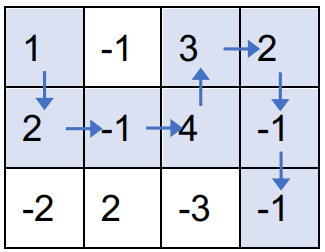
\includegraphics{num.png}\\
按上述走法,取到的数之和为 1 + 2 + (-1) + 4 + 3 + 2 + (-1) + (-1) = 9,可
以证明为最大值。\\
解:\\

\section{fruit-2021}
小熊的果篮(fruit)\\
【题目描述】\\
小熊的水果店里摆放着一排 n 个水果。每个水果只可能是苹果或桔子,从左到右依
次用正整数 1、 2、 3、 ……、 n 编号。连续排在一起的同一种水果称为一个“块”。小熊
要把这一排水果挑到若干个果篮里,具体方法是:每次都把每一个“块”中最左边的水
果同时挑出,组成一个果篮。重复这一操作,直至水果用完。注意,每次挑完一个果篮
后,“块”可能会发生变化。比如两个苹果“块”之间的唯一桔子被挑走后,两个苹果
“块”就变成了一个“块”。请帮小熊计算每个果篮里包含的水果。\\
【输入格式】\\
从文件 fruit.in 中读入数据。\\
输入的第一行包含一个正整数 n,表示水果的数量。\\
输入的第二行包含 n 个空格分隔的整数,其中第 i 个数表示编号为 i 的水果的种
类, 1 代表苹果, 0 代表桔子。\\
【输出格式】\\
输出到文件 fruit.out 中。\\
输出若干行。\\
第 i 行表示第 i 次挑出的水果组成的果篮。从小到大排序输出该果篮中所有水果的
编号,每两个编号之间用一个空格分隔。\\
【样例 1 输入】\\
\begin{tabular}{|c|}
\hline
12\\
1 1 0 0 1 1 1 0 1 1 0 0\\
\hline
\end{tabular}\\
【样例 1 输出】\\
\begin{tabular}{|c|}
\hline
1 3 5 8 9 11\\
2 4 6 12\\
7\\
10\\
\hline
\end{tabular}\\
【样例 1 解释】\\
这是第一组数据的样例说明。\\
所有水果一开始的情况是 1 1 0 0 1 1 1 0 1 1 0 0,一共有 6 个块。\\
在第一次挑水果组成果篮的过程中,编号为 1358911 的水果被挑了出来。\\
之后剩下的水果是 1 0 1 1 1 0,一共 4 个块。\\
在第二次挑水果组成果篮的过程中,编号为 24612 的水果被挑了出来。\\
之后剩下的水果是 1 1,只有 1 个块。\\
在第三次挑水果组成果篮的过程中,编号为 7 的水果被挑了出来。\\
最后剩下的水果是 1,只有 1 个块。\\
在第四次挑水果组成果篮的过程中,编号为 10 的水果被挑了出来。\\
解:\\

\section{point-2022-4}
【题目描述】\\
在一个二维平面内,给定$n$个整数点 ($x_i$, $y_i$),此外你还可以自由添加$k$个整数点。你在自由添加$k$个点后,还需要从$n+k$个点中选出若干个整数点并组成一个序列,使得序列中任意相邻两点间的欧几里得距离恰好为1而且横坐标、纵坐标值均单调不减,即$x_{i+1} −x_i=1$, $y_{i+1}=y_i$或$y_{i+1}−y_i=1$, $x_{i+1}=x_i$。请给出满足条件的序列的最大长度。\\
【输入格式】\\
从文件 point.in 中读入数据。\\
第一行两个正整数 n, k分别表示给定的整点个数、可自由添加的整点个数。接下来 n 行,第 i 行两个正整数 xi, yi 表示给定的第 i 个点的横纵坐标。\\
【输出格式】\\
输出到文件 point.out 中。\\
输出一个整数表示满足要求的序列的最大长度。\\
【样例 1 输入】\\
\begin{tabular}{|c|}
\hline
8 2\\
3 1\\
3 2\\
3 3\\
3 6\\
1 2\\
2 2\\
5 5\\
5 3\\
\hline
\end{tabular}\\
【样例 1 输出】\\
\begin{tabular}{|c|}
\hline
8\\
\hline
\end{tabular}\\
【样例 2 输入】\\
\begin{tabular}{|c|}
\hline
4 100\\
10 10\\
15 25\\
20 20\\
30 30\\
\hline
\end{tabular}\\
【样例 2 输出】\\
\begin{tabular}{|c|}
\hline
103\\
\hline
\end{tabular}\\
解:\\

\section{josephus-2021}
(Josephus 问题)有$n$个人围成一个圈,依次标号0至$�n-1$。\\
从0号开始,依次 0, 1, 0, 1, … 交替报数,报到 1 的人会离开,直至圈中只剩下一个人。\\
求最后剩下人的编号。\\
求解方法:\\
解决Josephus问题的经典方法是使用递归或数学公式。\\
可以得到一个递推关系式,用 f(n,m) 表示 n 个人报数,报到 m 时最后剩下的人的编号。\\
递推关系式为:\\
$f(n,m)=(f(n-1,m)+m)\%n$\\
其中,f(1,m) = 0,表示只剩下一个人时的情况。\\
这个关系式的意义是:在 n 个人报数的情况下,\\
第一轮报数时,第一个被淘汰的人的编号为 (f(n-1,m) + m) % n。\\
然后问题转化为 n-1 个人报数的情况,并从下一个人开始重新报数。\\
通过不断递归计算 f(n,m),最终可以得到只剩下最后一个人的编号,即 Josephus 问题的解。\\
解:\\
\begin{lstlisting}[language=c++,breaklines=true]
#include <iostream>

using namespace std;

const int MAXN = 1000000; // 最大的人数
int F[MAXN]; // 标记每个人是否被淘汰出圈

int main(){
	int n;
	cin >> n; // 接收输入的人数n
	int i = 0,p = 0,c = 0; // 当前报数的人编号、报数的标记、以及已经被淘汰的人数
	while(c < n - 1){ // 进入一个while循环,循环条件是还未剩下最后一个人
		if(F[i] == 0){ // 判断当前报数的人是否还在圈内,如果F[i]为0,表示该人还在圈内
			if(p){// 判断当前报数标记p的值。p的初始值为0,当p为1时,说明报数到1i,该人将被淘汰
				F[i] = 1; // 将当前报数的人标记为1,表示被淘汰
				c++; // 然后c增加1,表示已经淘汰的人数加1 
			} 
			p^=1; // 将p的值进行异或运算,相当于p取反,即0变成1,1变成0。这样可以实现交替报数的效果
		}
		i = (i + 1) % n; // 更新报数的人的编号i,取余操作确保编号在圈内循环
	}
	int ans = -1; // 定义一个变量ans,用于记录最后剩下的人的编号,初始化为-1
	for(i = 0;i < n;i++) // 遍历数组F,查找最后剩下的人的编号
		if(F[i] == 0) // 如果F[i]为0,表示该人未被淘汰
			ans = i; // 将该人的编号赋值给ans
	cout << ans << endl;
	return 0;
}
\end{lstlisting}

\clearpage
\end{document}
